\documentclass{beamer}
\usepackage{fontspec}
\usepackage{minted}
\usepackage{tango}
\usepackage{ccicons}
\usepackage{tikz}
\usepackage[normalem]{ulem}
\usepackage{csquotes}
\usepackage{amssymb}

\mode<presentation>{\usetheme{rwo}}
\title{Using static typing features for fun and profit}
\author{Marek~Kubica}
\date{6.~August~2013}
\institute{Lambda Munich}

\setsansfont{Yanone Kaffeesatz Regular}
\setmainfont{EB Garamond}
\setmonofont[Scale=0.8]{Droid Sans Mono Dotted}

\usemintedstyle{tango}
\setbeamerfont{title}{family=\rmfamily}

\setlength{\parskip}{8pt plus 1pt minus 1pt}

\defbeamertemplate*{title page}{rwo}[1][]
{
  \vbox{}
  \vfill
  \begin{centering}
    \begin{beamercolorbox}[sep=8pt,center,#1]{title}
      \usebeamerfont{title}\inserttitle\par%
      \ifx\insertsubtitle\@empty%
      \else%
        \vskip0.25em%
        {\usebeamerfont{subtitle}\usebeamercolor[fg]{subtitle}\insertsubtitle\par}%
      \fi%     
    \end{beamercolorbox}%
  \end{centering}
    \vskip1em\par
    \begin{beamercolorbox}[sep=3pt,#1]{author}
      \usebeamerfont{author}\insertauthor
    \end{beamercolorbox}
    \begin{beamercolorbox}[sep=3pt,#1]{institute}
      \usebeamerfont{institute}\insertinstitute
    \end{beamercolorbox}
    \begin{beamercolorbox}[sep=3pt,#1]{date}
      \usebeamerfont{date}\insertdate
    \end{beamercolorbox}\vskip0.5em
    {\usebeamercolor[fg]{titlegraphic}\inserttitlegraphic\par}
  \vskip4.0em
  \ccby{}\\
  {\tiny This work is licensed under a
  \href{http://creativecommons.org/licenses/by/3.0/deed.en_US}%
  {Creative Commons Attribution 3.0 Unported License}.}
  \vspace*{-2.5ex}
}


\renewcommand{\example}[1]{{\usebeamercolor[fg]{example text} #1}}
\renewcommand{\ULthickness}[0]{0.23ex}

\begin{document}

{
  \usebackgroundtemplate%
  {%
    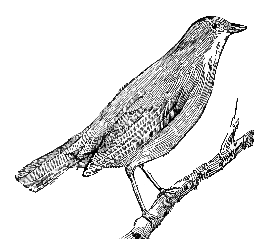
\includegraphics[width=\paperwidth,height=\paperheight]{nightingdale}%
  }
  \frame{\titlepage}
}

\begin{frame}
  \begin{alertblock}{Disclaimer}
    I am not a professional OCaml programmer, type theoretician etc.
  \end{alertblock}
  \pause
  \begin{alertblock}{Static typing?}
    I am neither a static typing weenie, I like dynamically typed languages
    too, so put your flamewar away (for now).
  \end{alertblock}
\end{frame}

\begin{frame}{Who am I?}
  \begin{columns}
    \column{0.4\textwidth}
      \begin{itemize}
        \item Marek Kubica
        \item Student at the TUM
        \item I do free software
        \item Dabbled in just about every language evar
      \end{itemize}
    \column{0.6\textwidth}
      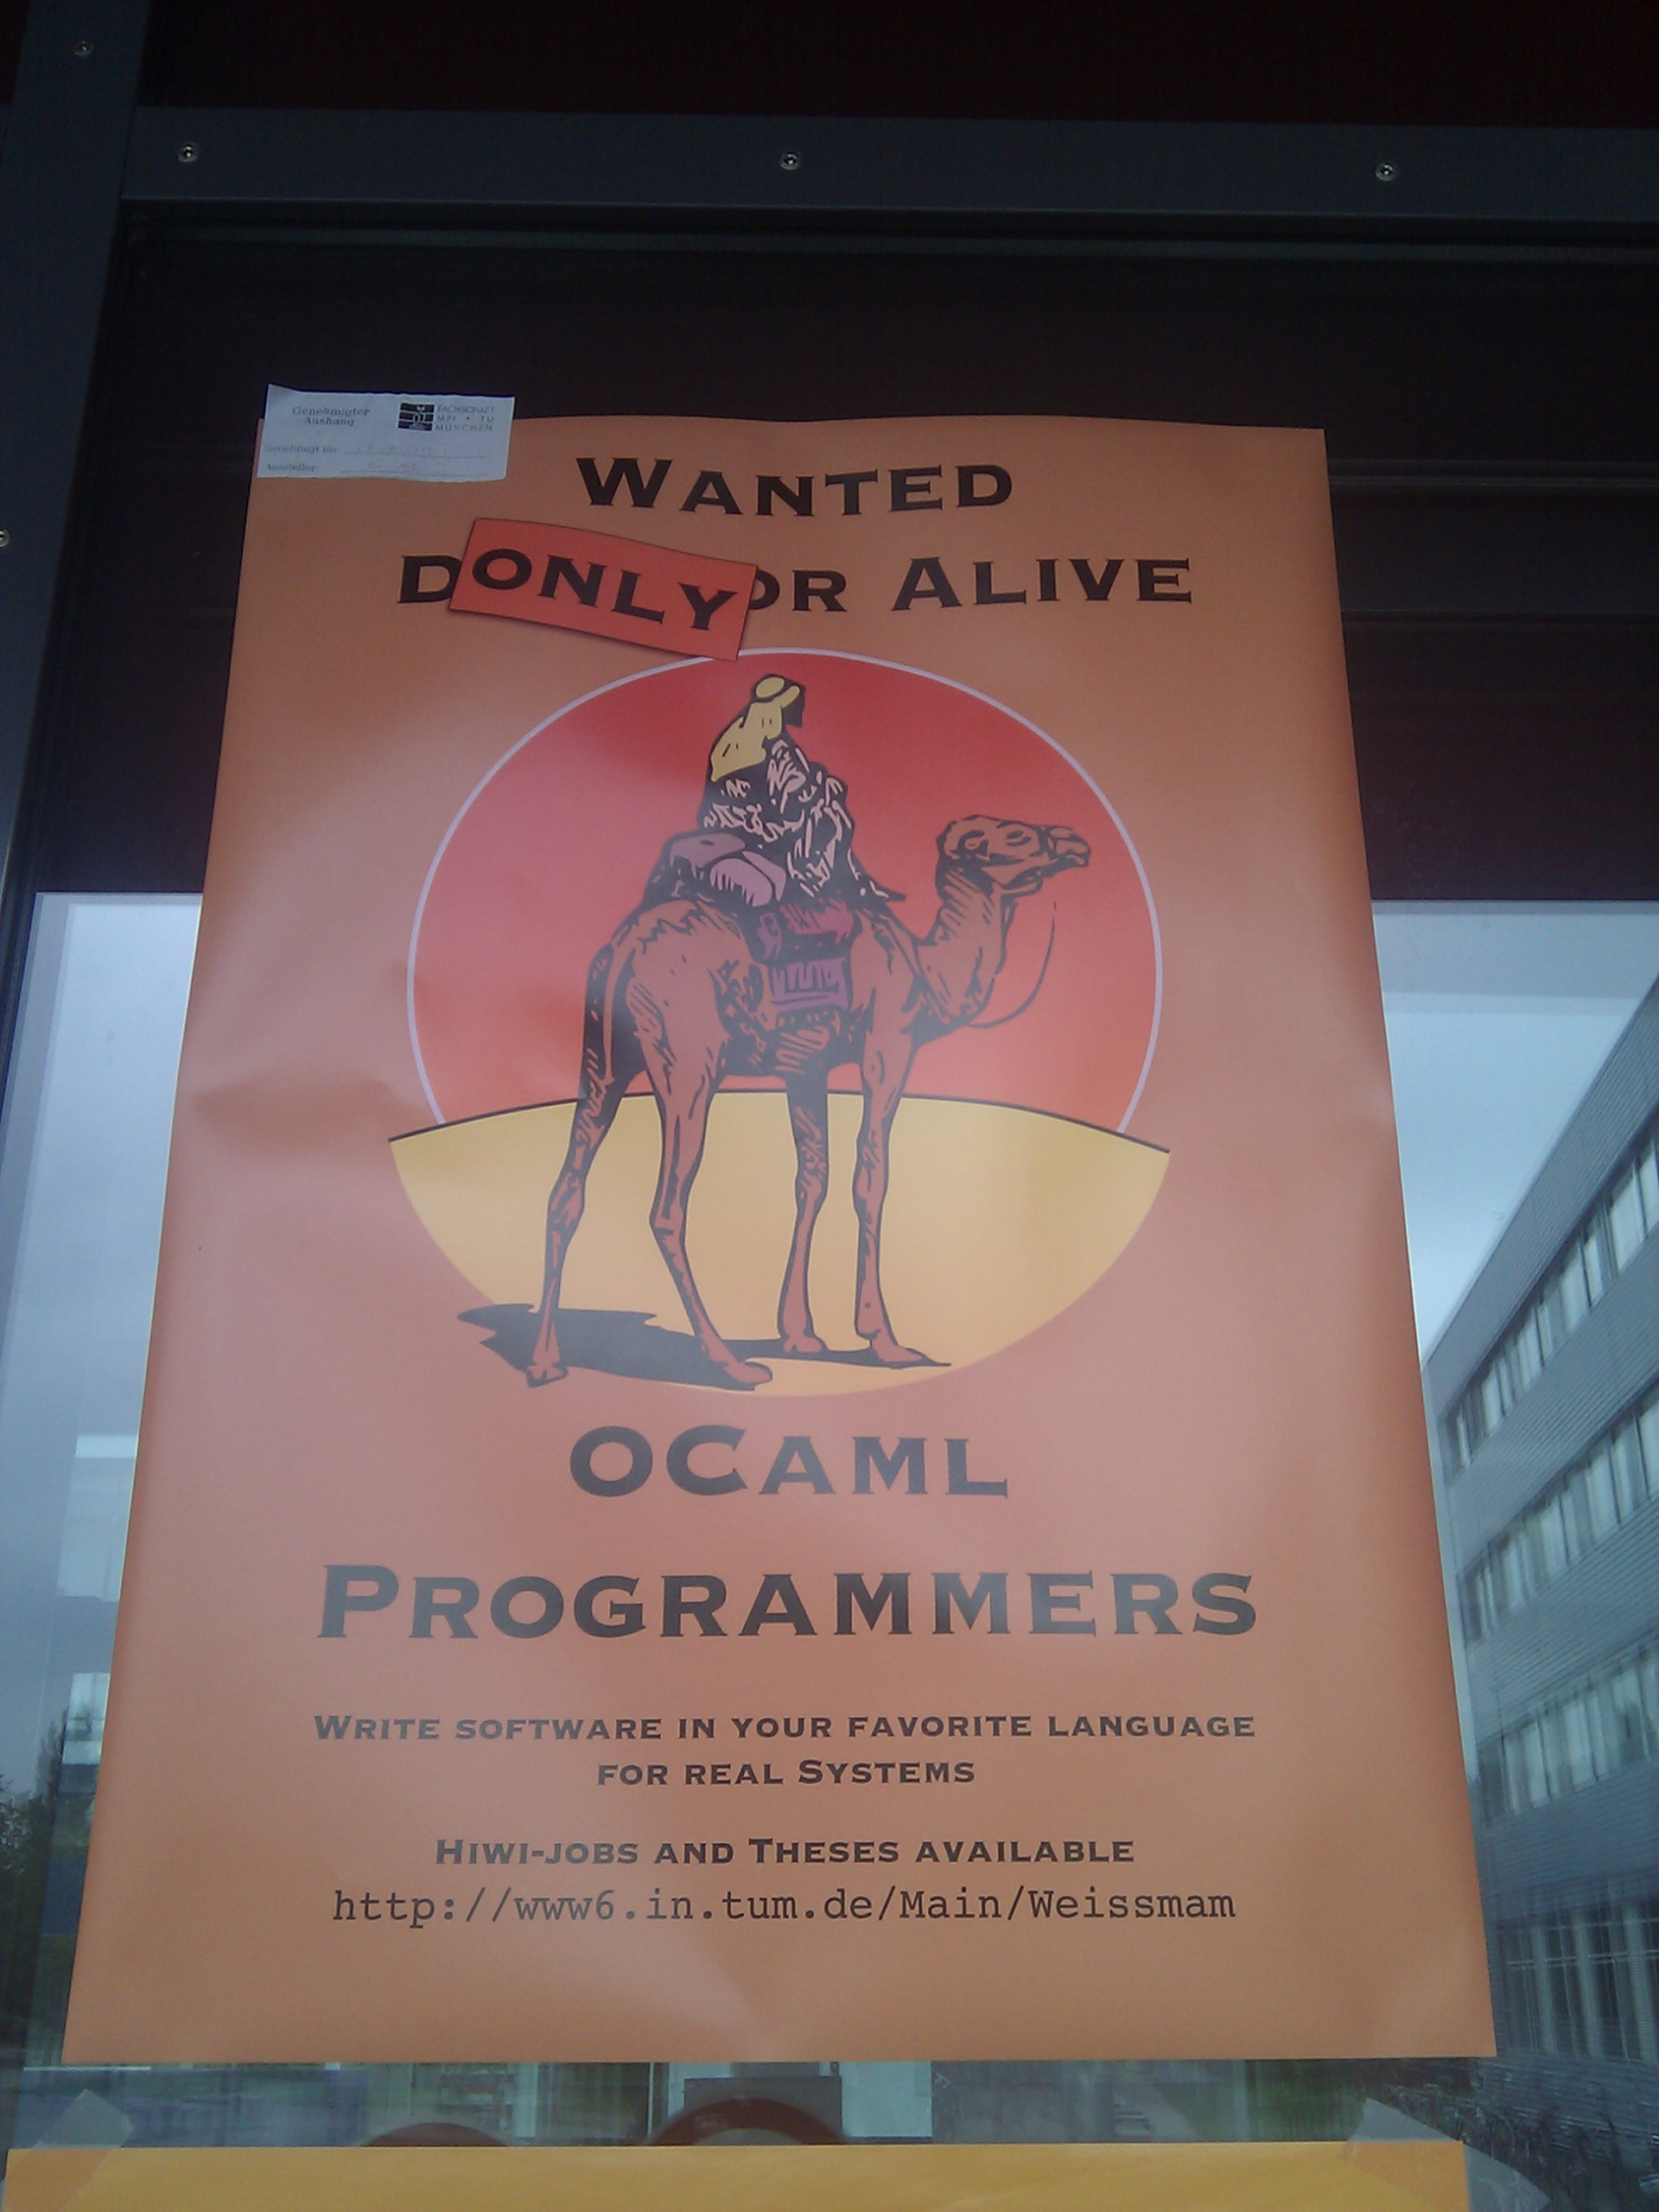
\includegraphics[height=0.9\textheight]{poster}
  \end{columns}
\end{frame}

\begin{frame}
  \begin{itemize}
    \item Data compression support in OCaml is… kinda meh
    \item Using OCaml FFI to interface to libarchive
    \item Thought I might as well create a better API
    \item What IS a better API anyway?
  \end{itemize}
  \pause
  \begin{exampleblock}{My goal for tonight}
    Show you that advanced static type features are not (only) academic.
  \end{exampleblock}
\end{frame}

\begin{frame}[fragile]{Static typing the C way}
  Let's check how C handles look like. How about checking libarchive.
  \begin{minted}[gobble=4]{c}
    __LA_DECL struct archive* archive_read_new(void);
    __LA_DECL struct archive* archive_write_new(void);
  \end{minted}
  \begin{itemize}
    \item Opaque pointer to some struct
    \item Write handles and read handles have the same type
  \end{itemize}
\end{frame}

\begin{frame}
  So, what can we do with these handles?
  \pause
  \begin{itemize}
    \item Create them
    \item Open them
    \item Configure them
    \item Read from them
    \item Write to them
    \item Close them
  \end{itemize}
  \pause
  Cool.
  \pause
  \alert{But what if we screw up?}
\end{frame}

\begin{frame}[fragile]{Segfault}
  \begin{minted}[gobble=4]{text}
    zsh: segmentation fault (core dumped)  ./errors
  \end{minted}
\end{frame}

\begin{frame}[fragile]{Double free}
\begin{minted}[fontsize=\tiny]{text}
*** Error in `./errors': double free or corruption (fasttop): 0x000000000077a010 ***
======= Backtrace: =========
/usr/lib/libc.so.6(+0x788ae)[0x7fa0c97cd8ae]
/usr/lib/libc.so.6(+0x79587)[0x7fa0c97ce587]
./errors[0x40057b]
/usr/lib/libc.so.6(__libc_start_main+0xf5)[0x7fa0c9776a15]
./errors[0x400479]
======= Memory map: ========
00400000-00401000 r-xp 00000000 fe:01 21244012                           /home/marek/lambda-munich/errors
00600000-00601000 rw-p 00000000 fe:01 21244012                           /home/marek/lambda-munich/errors
0077a000-0079b000 rw-p 00000000 00:00 0                                  [heap]
7fa0c953f000-7fa0c9554000 r-xp 00000000 fe:00 4213606                    /usr/lib/libgcc_s.so.1
7fa0c9554000-7fa0c9754000 ---p 00015000 fe:00 4213606                    /usr/lib/libgcc_s.so.1
7fa0c9754000-7fa0c9755000 rw-p 00015000 fe:00 4213606                    /usr/lib/libgcc_s.so.1
7fa0c9755000-7fa0c98f8000 r-xp 00000000 fe:00 4202529                    /usr/lib/libc-2.17.so
7fa0c98f8000-7fa0c9af8000 ---p 001a3000 fe:00 4202529                    /usr/lib/libc-2.17.so
7fa0c9af8000-7fa0c9afc000 r--p 001a3000 fe:00 4202529                    /usr/lib/libc-2.17.so
7fa0c9afc000-7fa0c9afe000 rw-p 001a7000 fe:00 4202529                    /usr/lib/libc-2.17.so
7fa0c9afe000-7fa0c9b02000 rw-p 00000000 00:00 0 
7fa0c9b02000-7fa0c9b23000 r-xp 00000000 fe:00 4203728                    /usr/lib/ld-2.17.so
7fa0c9cfa000-7fa0c9cfd000 rw-p 00000000 00:00 0 
7fa0c9d22000-7fa0c9d23000 rw-p 00000000 00:00 0 
7fa0c9d23000-7fa0c9d24000 r--p 00021000 fe:00 4203728                    /usr/lib/ld-2.17.so
7fa0c9d24000-7fa0c9d25000 rw-p 00022000 fe:00 4203728                    /usr/lib/ld-2.17.so
7fa0c9d25000-7fa0c9d26000 rw-p 00000000 00:00 0 
7fff44461000-7fff44482000 rw-p 00000000 00:00 0                          [stack]
7fff445fe000-7fff44600000 r-xp 00000000 00:00 0                          [vdso]
ffffffffff600000-ffffffffff601000 r-xp 00000000 00:00 0                  [vsyscall]
zsh: abort (core dumped)  ./errors foo
\end{minted}
\end{frame}

\begin{frame}
  What actually happens: libarchive returns \texttt{ARCHIVE\_FATAL}.\pause

  Unless you trigger a bug in libarchive. \pause
  \alert{Then it segfaults.}
\end{frame}

\begin{frame}{Lots of things can go wrong}
  \begin{itemize}
    \item Reading from handle that is not open *
    \item Writing to a read handle
    \item Not setting the options correctly (compression formats)
  \end{itemize}
  \pause
  * this actually happened
\end{frame}

\begin{frame}{Not to gripe on libarchive}
  \begin{exampleblock}{Public Service Announcement}
    libarchive is a rather well designed library. Rather idiomatic C, so don't
    think this is a deliberately bad example. It is how things are in C land.
  \end{exampleblock}

  \begin{itemize}
    \item This is an OK API for C.
    \item Fragile APIs are common in C.
  \end{itemize}

  \vspace{2ex}
  \pause
  \begin{center}
    {\Large But can we do better?}
  \end{center}
\end{frame}

\begin{frame}
  \begin{center}
    {\fontsize{56pt}{54pt}\selectfont \example{Yes}}\\
    \pause
    {\scriptsize (obviously)}
  \end{center}
\end{frame}

\begin{frame}[fragile]{Fix up the handle types}
  How to prevent writing to read handles and reading from write handles?
  \begin{minted}[gobble=4]{ocaml}
    external read_new: unit -> archive = "ost_read_new"
    external write_new: unit -> archive = "ost_write_new"
  \end{minted}
  \pause
  Yup, create different handle types.
  \begin{minted}[gobble=4]{ocaml}
    type r = archive
    type w = (archive * write_buffer_ptr * written_ptr)
  \end{minted}
  So now we have two different types to represent handles.
\end{frame}

\begin{frame}{Achivement unlocked!}
  \begin{center}
    {\Huge Type safety improved!}
  \end{center}
  \checkmark Writing read handles disallowed

  But of course you aren't attending the talk for this \alert{trivial}
  epiphany. We can do this easily in C as well! Let's do better.
\end{frame}

\begin{frame}[fragile]{Our handles have states!}
  The handles always traverse some fixed states:
\begin{center}
% dot2tex --figonly states.dot
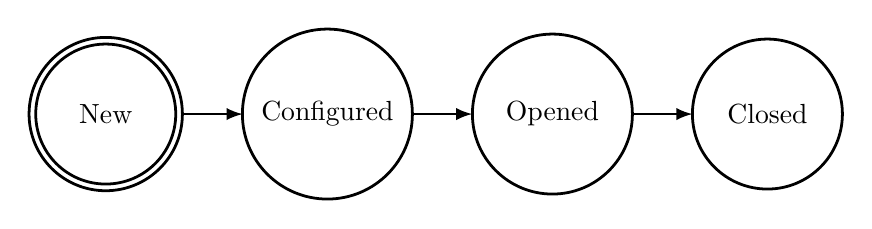
\begin{tikzpicture}[>=latex,line join=bevel,scale=0.6]
  \pgfsetlinewidth{1bp}
%%
\pgfsetcolor{black}
  % Edge: New -> Configured
  \draw [->] (92.45bp,50bp) .. controls (100.74bp,50bp) and (109.5bp,50bp)  .. (128.16bp,50bp);
  % Edge: Opened -> Closed
  \draw [->] (362.29bp,50bp) .. controls (370.61bp,50bp) and (379.33bp,50bp)  .. (398.03bp,50bp);
  % Edge: Configured -> Opened
  \draw [->] (229.9bp,50bp) .. controls (238.38bp,50bp) and (247.24bp,50bp)  .. (265.9bp,50bp);
  % Node: New
\begin{scope}
  \definecolor{strokecol}{rgb}{0.0,0.0,0.0};
  \pgfsetstrokecolor{strokecol}
  \draw (46bp,50bp) ellipse (42bp and 42bp);
  \draw (46bp,50bp) ellipse (46bp and 46bp);
  \draw (46bp,50bp) node {   New};
\end{scope}
  % Node: Configured
\begin{scope}
  \definecolor{strokecol}{rgb}{0.0,0.0,0.0};
  \pgfsetstrokecolor{strokecol}
  \draw (179bp,50bp) ellipse (51bp and 51bp);
  \draw (179bp,50bp) node {Configured};
\end{scope}
  % Node: Opened
\begin{scope}
  \definecolor{strokecol}{rgb}{0.0,0.0,0.0};
  \pgfsetstrokecolor{strokecol}
  \draw (314bp,50bp) ellipse (48bp and 48bp);
  \draw (314bp,50bp) node {  Opened};
\end{scope}
  % Node: Closed
\begin{scope}
  \definecolor{strokecol}{rgb}{0.0,0.0,0.0};
  \pgfsetstrokecolor{strokecol}
  \draw (443bp,50bp) ellipse (45bp and 45bp);
  \draw (443bp,50bp) node {  Closed};
\end{scope}
%
\end{tikzpicture}
\end{center}
Couldn't we \example{encode the state} in the type somehow?
\end{frame}

\begin{frame}[fragile]{Adding state information in the type}
  We can add state. OCaml has parametrized types *:

  \begin{minted}[gobble=4]{ocaml}
    # [];;
    - : 'a list = []
    # [1];;
    - : int list = [1]
    # type 'a read_handle = ReadHandle of 'a;;
    type 'a read_handle = ReadHandle of 'a
  \end{minted}

  * if you haven't seen them, think of them kinda like generics
\end{frame}

\begin{frame}[fragile]{Aside: Open union types}
  So, now we can \example{parametrize types with other types}.

  We could create our own state types:
  \begin{minted}[gobble=4]{ocaml}
    type state = New | Configured | Opened | Closed
  \end{minted}
  \pause
  But these \alert{can't be extended} if someone wants to add a new state.
  \pause

  Plus, we're lazy. Let's use \example{open union types} aka polymorphic variants:
  \begin{minted}[gobble=4]{ocaml}
    [`New] [`Configured] [`Opened] [`Closed]
  \end{minted}
\end{frame}

\begin{frame}
  Great, so now we can create functions that take handles of the correct state.

  e.g. a read function that only works on \texttt{[`Opened] read\_handle}.

  \pause
  \alert{Foiled again!}
  \pause

  The OCaml compiler is too smart, it knows that \texttt{[`Opened] read\_handle} is the
  same type as \texttt{[`New] read\_handle} therefore every function which takes
  the \texttt{[`Opened]} handle takes every other type too.
\end{frame}

\begin{frame}[fragile]{Enter phantoms}
  We'd need to \alert{hide} the actual \texttt{read\_handle} type from the compiler.

  \pause

  Boy oh boy, we can!

  \pause

  We create a module and only say:
  \begin{minted}{ocaml}
  module Handle : sig
    type 'a r
    (* our signatures *)
    val new : unit -> [`New] r
  end = struct
    type 'a r = read_handle
    (* our functions *)
    external new : unit -> [`Open] r = "ost_read_new"
  end
  \end{minted}
\end{frame}

\begin{frame}{Achivement unlocked!}
  \begin{center}
    {\Huge Made API misuse a type error!}
  \end{center}
  \checkmark Writing read handles disallowed\\
  \checkmark Using the proper handle in an incorrect way disallowed
\end{frame}

\begin{frame}
  \begin{center}
    {\Huge And now for something completely different!}
  \end{center}
\end{frame}

\begin{frame}[fragile]{Have you ever seen this?}
  Ever used Python?
  \begin{minted}[gobble=4]{text}
    Traceback (most recent call last):
    File "<stdin>", line 1, in <module>
    AttributeError: 'NoneType' object has no attribute 'foo'
  \end{minted}
  \pause
  Ever touched Java?
  \begin{minted}[gobble=4]{text}
    Exception in thread "main" java.lang.NullPointerException
    at NPE.main(NPE.java:8)
  \end{minted}
  \pause
  Ever seen C?
  \begin{minted}[gobble=4]{text}
    zsh: segmentation fault (core dumped)  ./errors
  \end{minted}
\end{frame}

\begin{frame}{You know whose fault it is!}
  \begin{itemize}
    \item \texttt{null}
    \item \texttt{None}
    \item \texttt{NULL}
  \end{itemize}
  \pause
  Everytime you return null as a placeholder value, 
  \sout{\textdollar{}DEITY kills a kitten}
  you have to check whether you weren't handed null in return.
\end{frame}

\begin{frame}
  \begin{center}
    {\Huge Let's kill the \sout{Batman} Null pointer!}
  \end{center}
\end{frame}

\begin{frame}{Attempt one: Exceptions}
  \begin{itemize}
    \item Common solution
    \item Ubiquitous (Java, Python, C++, Ruby, whathaveyou)
    \item Easy to understand
    \item OCaml does have exceptions
    \pause
    \item \alert{Not typesafe}, unless you consider checked exceptions
    \item Boring!
  \end{itemize}
\end{frame}

\begin{frame}[fragile]{Attempt two: Option types}
  Observation: everythime we return NULL, we either return something
  meaningful or an invalid placeholder.

  We might even say:
  \begin{minted}[gobble=4]{ocaml}
    type 'a option = Some of 'a | None
  \end{minted}

  \pause

  Therefore, everytime a function returns \texttt{'a option} we have
  to pattern match:
  \begin{minted}[gobble=4]{ocaml}
    let optional x = Some x
    match optional 42 with
      | Some x -> x
      | None -> 0
  \end{minted}

  \pause

  If we forget:
  \begin{minted}[gobble=4]{text}
    Warning 8: this pattern-matching is not exhaustive.
    Here is an example of a value that is not matched:
    None
  \end{minted}
\end{frame}

\begin{frame}{Achivement unlocked!}
  \begin{center}
    {\Huge Forgetting to check for NULL is a type error!}
  \end{center}
  \checkmark No more Null pointer failures on runtime!
\end{frame}

\begin{frame}[fragile]
  Everything is fun and games until you need to specify a \alert{reason} for
  failure.

  What if we could add an error message?
  \begin{minted}[gobble=4]{ocaml}
    type ('a, 'b) err = Success of 'a | Failure of 'b
  \end{minted}
  Done!
\end{frame}

\begin{frame}[fragile]
  But pattern matching on every function call sucks because it is
  \alert{tedious}! Just look at this mess:
  \begin{minted}[gobble=4]{ocaml}
    match firstfn 42 with 
      | Success (x) -> (match secondfn x with
        | Success (y) -> (match thirdfn y with
          | Success (z) -> z
          | Failure (f3) -> "Failure at thirdfn")
        | Failure (f2) -> "Failure at secondfn")
      | Failure (f1) -> "Failure at fristfn"
  \end{minted}

  Right. Maybe we can \example{simplify}…

  In Haskell, \texttt{option} is called \enquote{Maybe monad} and 
  \texttt{error} is called \enquote{Error monad}.

  \pause
  \begin{center}
    {\Large \alert{BAM, SCARY MONADS!}}
  \end{center}
\end{frame}

\begin{frame}[fragile]
  Haskell features an operator called \texttt{bind} aka \texttt{>>=} to
  chain operations on monads.

  \begin{minted}[gobble=4]{ocaml}
    val bind: 'a ErrorMonad.t -> ('a -> 'b ErrorMonad.t) ->
      'b ErrorMonad.t
  \end{minted}

  \texttt{bind} takes an error monad wrapping type \texttt{'a}, and a function
  which takes \texttt{'a} and returns an error monad wrapping
  \texttt{'b} and returns that value.

  Basically an unwrapper function.
\end{frame}

\begin{frame}[fragile]
  For the error monad, it looks like this:
  \begin{minted}[gobble=4]{ocaml}
    let bind m f = match m with
      | Success(x) -> f x
      | Failure(f) -> Failure(f)
  \end{minted}

  We can use it like this:

  \begin{minted}[gobble=4]{ocaml}
    match (bind (bind (firstfn 42) secondfn) thirdfn) with
      | Success (x) -> x
      | Failure (_) -> "Failure in chain"
  \end{minted}
  The code got a lot \example{easier}!
\end{frame}

\begin{frame}[fragile]{Aside: Operator tricks}
  OCaml allows \alert{custom operators} as long as they follow naming rules.

  \begin{minted}[gobble=4]{ocaml}
    let (>>=) = bind
  \end{minted}

  Using it is \example{easy}:

  \begin{minted}[gobble=4]{ocaml}
    match (firstfn 42) >>= secondfn >>= thirdfn with
      | Success (x) -> x
      | Failure (_) -> "Failure in chain"
  \end{minted}
\end{frame}

\begin{frame}{Achivement unlocked!}
  \begin{center}
    {\Huge Statically typed error handling}
  \end{center}
  \checkmark No more Null pointer failures on runtime!\\
  \checkmark Easy and convenient to get reason of failure
\end{frame}

% last slide, in any case
{
\usebackgroundtemplate{
\includegraphics[height=\paperheight]{instacode}}%
\begin{frame}[plain]
  \begin{columns}
    \column{0.5\textwidth}
  \begin{block}{Marek Kubica}
    Check out my playthings:
    \begin{itemize}
      \item \href{https://github.com/Leonidas-from-XIV}{Leonidas-from-XIV} on GitHub
      \item Leonidas nearly everywhere else
      \item \url{http://xivilization.net/}
    \end{itemize}
  \end{block}
    \column{0.5\textwidth}
      % nothing
  \end{columns}
\end{frame}
}

\end{document}
